\documentclass[a4paper,12pt]{article} % тип документа

%%% Работа с русским языком
\usepackage{cmap}					% поиск в PDF
\usepackage{mathtext} 				% русские буквы в фомулах
\usepackage[T2A]{fontenc}			% кодировка
\usepackage[utf8]{inputenc}			% кодировка исходного текста

\usepackage[english,russian]{babel}	% локализация и переносы
\usepackage[left= 2 cm,right= 2 cm,
    top=2cm,bottom=4cm,bindingoffset=0cm]{geometry} %настройка полей и отступов снерху/снизу листа
    \usepackage[argument]{graphicx}
    \usepackage{graphicx}

    \usepackage[table,xcdraw]{xcolor} % возможность создания таблиц с цветными ячейками
    %\usepackage{indentfirst}
   
\graphicspath{{./pictures/}}  % папки с картинками
\setlength\fboxsep{3pt} % Отступ рамки \fbox{} от рисунка
\setlength\fboxrule{1pt} % Толщина линий рамки \fbox{}
\usepackage{wrapfig} % Обтекание рисунков и таблиц текстом
    

%%% Дополнительная работа с математикой
\usepackage{amsmath,amsfonts,amssymb,amsthm,mathtools} % AMS
\usepackage{icomma} % "Умная" запятая: $0,2$ --- число, $0, 2$ --- перечисление

%% Номера формул
\mathtoolsset{showonlyrefs=true} % Показывать номера только у тех формул, на которые есть \eqref{} в тексте.

%% Шрифты
\usepackage{euscript}	 % Шрифт Евклид
\usepackage{mathrsfs} % Красивый матшрифт

%% Свои команды
\DeclareMathOperator{\sgn}{\mathop{sgn}}

%% Перенос знаков в формулах (по Львовскому)
\newcommand*{\hm}[1]{#1\nobreak\discretionary{}
{\hbox{$\mathsurround=0pt #1$}}{}}

\title{Тамэси-вари}
\author{Гончаренко Валентина, 1 курс ФРКТ, группа Б01-009}
\date{Январь 2021}

\begin{document}

\maketitle
\thispagestyle{empty} % нумерация выкл.

\newpage
\begin{center}
\section*{Сначала было каратэ...}
\end{center}
Тамэси-вари - это проверка психологической подготовки и техники удара в каратэ различных предметов. Известно, что каратэ пришло к нам с Окинавы, крупнейшего острова Японии. Наибольшее развитие каратэ получило в 16-17 веках, когда власти, опасаясь восстаний, изъяли у населения все оружие, включая кухонные ножи и церемониальные мечи. Конечно, сопротивляться хорошо вооруженной армии самураев голыми руками крестьянам было не под силу, но, зная приёмы каратэ, они могли дать отпор нескольким оголтелым насильникам. Видимо, отсюда и берет начало практика тамэси-вари, которая всегда интересна для зрителей и производит на непосвященных впечатление некоторого чуда. В наше время на показательных выступлениях и соревнованиях по каратэ в тамэси-вари чаще всего используются доски определенных размеров из деревьев хвойных пород.

Когда я выбирала тему вопроса по выбору, я просматривала архивы физических статей в журнале "Квант". Среди многих названий более-менее знакомых терминов, которые интуитивно можно было отнести к разделу механики, я увидела необычное слово, никогда раньше мне не попадавшееся (более того, я до сих пор не знаю правильной постановки ударения в нём, потому что нигде это не отыскала). Нажав на ссылку, я удивилась и обрадовалась, так как статья показалась наиболее интересной для детального разбора. Мне, как и автору, стало интересно исследовать характерные параметры и значения для этой техники удара, если не брать во внимание психологический аспект вопроса. В связи с этим была рассмотрена физическая модель удара по доске, которая позволяет сделать некоторые расчеты и оценить возможности человека в тамэси-вари. Определение ряда величин этой модели требует решения нескольких самостоятельных задач, которые вынесены в Приложения (1-3) для более наглядного изложения основного текста.

\newpage
\begin{wrapfigure}[9]{r}{0.4\linewidth}
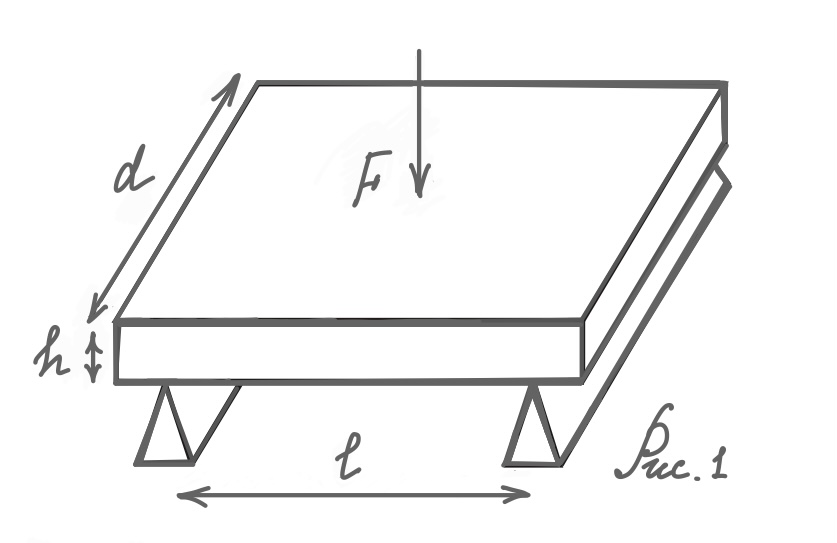
\includegraphics[width=7cm]{pictures/1.PNG}
\label{fig:image}
\end{wrapfigure}
Пусть по центру лежащей на двух опорах доски с размерами ${d, l, h}$ (рис.1) наносят удар кулаком массой $m$ со скоростью $v$ в момент контакта. Волокна доски направлены параллельно опорам, расстояние между которыми для оценки также будем полагать равным длине доски $l$. Из <<секретов>> каратэ известно, что для увеличения эффективности удара надо к уже разогнанному перед ударом кулаку в течение времени его взаимодействия с доской прикладывать еще и силу, которую обозначим через $F$. Введем систему координат так, как показано на рисунке 2. Обозначим через $x_0$ смещение центра доски из положения равновесия. Пусть разрыв доски, т.е. разрыв ее внешней поверхности, происходит при некотором значении $x_0 = x_p$. Такой разрыв происходит, когда напряжение $\sigma$ (сила, действующая на единицу площади сечения доски) на поверхности доски достигает определенного значения $\sigma_p$, характеризующего материал.

Найдем вначале связь между $x_p$ и $\sigma_p$, которая, очевидно, определяется упругими свойствами и геометрическими размерами доски. Максимальный изгиб и, следовательно, максимальное напряжение на поверхности доски будет в ее середине. \begin{wrapfigure}[13]{l}{0.46\linewidth}
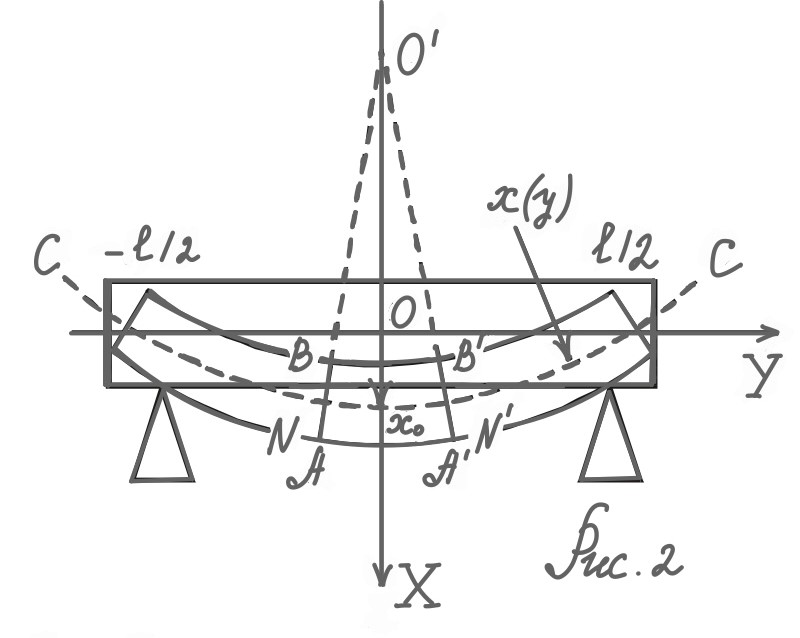
\includegraphics[width=8cm]{pictures/2.PNG}
\label{fig:image}
\end{wrapfigure}
Как показано в Приложении 1, это напряжение равно $\sigma$ = $\dfrac{Eh}{2R}$ , где \textit{R} - это радиус кривизны центральной линии \textit{CC} в середине доски (см. рис. 2), а \textit{E} - модуль Юнга материала доски. 

Зададим теперь форму доски при изгибе, учитывая, что края доски закреплены в точках $y$ = $\pm \dfrac{l}{2}$, а максимальное смещение из положения равновесия имеет её центр. Отметим, что точная форма доски зависит от конкретных условий контакта ударной поверхности кулака с доской (при правильном ударе - это суставы указательного и среднего пальцев). Поэтому для расчетов можно ограничиться удобной формулой, основанной на практическом опыте и позволяющей провести простые оценки. Будем считать форму доски при изгибе косинусоидой, закрепленной в точках $y$ = $\pm \dfrac{l}{2}$. В этом случае смещение $x$ какой-либо точки центральной линии зависит от её координаты $y$ по закону $$x(y) = x_0 \cos{\left(\dfrac{\pi y}{l}\right)}.$$

В Приложении 2 показано, что при этом радиус кривизны в центре доски будет равен $$R = \left(\dfrac{l}{\pi}\right)^2 \dfrac{1}{x_0}.$$

Подставив полученное выражение для радиуса кривизны в выражение для $\sigma$, найдем напряжение в середине доски на её поверхности при смещении центра доски на величину $x_0$: $$\sigma = \dfrac{x_0Eh\pi^2}{2l^2}.$$

Отсюда видно, что разлом ($\sigma$ = $\sigma_p$) происходит при смещении центра доски на величину $$x_p = \dfrac{2\sigma_pl^2}{\pi^2Eh}.$$

Смоделируем далее упругие свойства доски относительно приложенной внешней силы пружиной жесткостью $k$. Этот коэффициент найден в Приложении 3 и имеет величину $$k = \dfrac{\pi^2Eh^3d}{3l^3}.$$

После определения необходимых параметров вернемся к сформулированной раньше динамической задаче об ударе по доске и запишем уравнение движения кулака в виде второго закона Ньютона: $$mx'' = -kx + F,$$ где $x$ теперь - смещение кулака от исходной поверхности контакта с доской, а штрихи обозначают производные по времени. Для оценки будем полагать, что приложенная человеком к кулаку сила $F$ постоянна во времени. Непосредственной подстановкой можно убедиться, что общее решение уравнения движения имеет вид $$x = A\cos{\omega t} + B\sin{\omega t} + \dfrac{F}{k}$$ и содержит две произвольные константы $A$ и $B$. Для их определения зададим условия в начальный момент времени $t = 0$: $x = 0$ и $x' = v$. Тогда получим $$x = \dfrac{f}{\omega^2}(1 - \cos{\omega t}) + \dfrac{v}{\omega}\sin{\omega t},$$ где $f = \dfrac{F}{m}$ - величина, имеющая размерность ускорения, и $w = \sqrt{\dfrac{k}{m}}$ - частота собственных колебаний кулака под действием упругой силы со стороны доски. Найдем теперь максимальное отклонение кулака $x_{max}$ при заданном значении начальной скорости $v$ и силы $F$. Приравнивая к нулю производную от $x$ по времени $t$ и затем исключая $t$, находим $$x_{max} = \dfrac{f}{\omega^2}\left(1 + \sqrt{1 + \left(\dfrac{v\omega}{f}\right)^2}\right).$$ Для получения условий разлома это отклонение нужно приравнять к отклонению $x_p$, откуда получаем уравнение $$\dfrac{2\sigma_ph^2d}{3Fl} = 1 + \sqrt{1 + \dfrac{\pi^2Eh^3v^2dm}{3F^2l^3}},$$ связывающее свойство материала доски и её геометрические размеры с параметрами, характеризующими удар.

Решим это уравнение относительно силы $F$, опять вводя для удобства значения $x_p$ и $k$. В этих обозначениях получим простое выражение $$F = \dfrac{kx_p}{2} - \dfrac{mv^2}{2x_p}.$$ Tакую силу необходимо приложить в момент контакта к кулаку, движущемуся с начальной скоростью $v$, чтобы разбить доску. Очевидно, что, если скорость кулака достаточно велика, выражение для $F$ получается отрицательным и силу можно не прикладывать. В этом случае начальная скорость должна превышать значение $$v = x_pw = \dfrac{2\sigma_p}{\pi\sqrt{3}}\sqrt{\dfrac{lhd}{mE}},$$ которое пропорционально квадратному корню из толщины доски $h$. Наоборот, если начальная скорость кулака $v$ равна нулю, то из выражения для $F$ следует, что, для того чтобы сломать (продавить) доску, необходимо приложить силу $$F = \dfrac{kx_p}{2} = \dfrac{h^2\sigma_pd}{3l},$$ пропорциональную квадрату толщины $h$. Значит, с увеличением толщины доски выгоднее увеличивать скорость, а не силу.

Решим теперь уравнение, определяющее условие разлома доски относительно $h$ и получим значение толщины доски, которую можно разбить при заданных параметрах удара: $$h = \dfrac{3\pi^2Ev^2m}{8{\sigma_p}^2ld}\left(1 + \sqrt{1 + \dfrac{64Fl^3{\sigma_p}^3d}{3\pi^4E^2v^4m^2}}\right).$$

Проведем некоторые численнные оценки, задав характерные параметры материала доски: $E = 10^8$ H$/м^2$ и $\sigma_p = 5\cdot10^6$ H$/м^2$, взятые из экспериментальных измерений. Стандартные в тамэси-вари ширина и длина доски составляют 20 см и 30 см, однако в расчетах будем полагать $l = 25$ см, поскольку края доски, выступающие за опоры, можно не учитывать. Массу кулака с учетом предплечья можно положить равной 1 кг. На рисунке 3 показана зависимость силы $F$ от начальной скорости $v$ при различных значениях толщины доски $h$. Если сила и скорость таковы, что соответствующая точка лежит выше кривой для заданного $h$, то доска ломается.

Теперь оценим толщину доски, которую может сломать человек. \begin{wrapfigure}[13]{r}{0.47\linewidth}
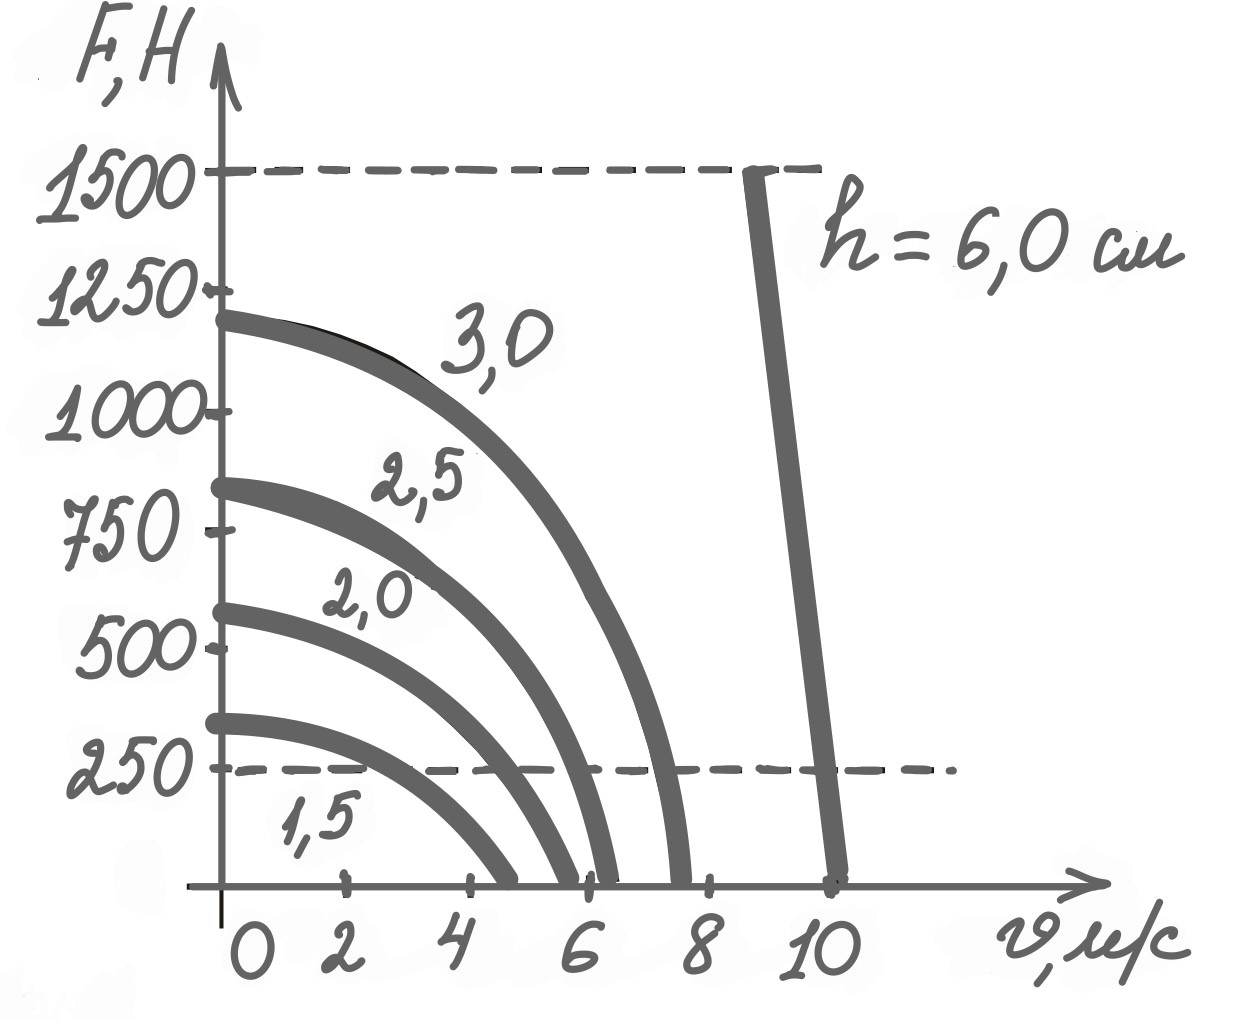
\includegraphics[width=7cm]{pictures/3.PNG}
\label{fig:image}
\end{wrapfigure}
Примем реальную cилу одной руки обычного человека равной $F = 250$ H. Как видно из рисунка, продавить такой силой (показана пунктиром) даже достаточно тонкую доску толщиной 1,5 см при начальной скорости $v = 0$ обычному человеку невозможно. Для этого необходимо развить силу около 300 H. Экспериментальное значение максимальной скорости удара кулаком оценивается как 10 м/с. Подставив в выражение для $h$ значение $v = 10$ м/с и $F = 250$ H, находим толщину доски: $h = 6$ см. Эта величина достаточно большая и доступная, по-видимому, только для тренированных людей, обладающих высокой техникой удара и психологически подготовленных.

\newpage
\section*{Приложение 1}

Определим напряжение на поверхности доски. Проведем (см. рис.2) симметричные сечения доски $AB$ и $A'B'$, нормальные к линии $CC$ и находящиеся на малом расстоянии $l_0$ друг от друга вдоль этой линии. 

\begin{wrapfigure}[14]{r}{0.45\linewidth}
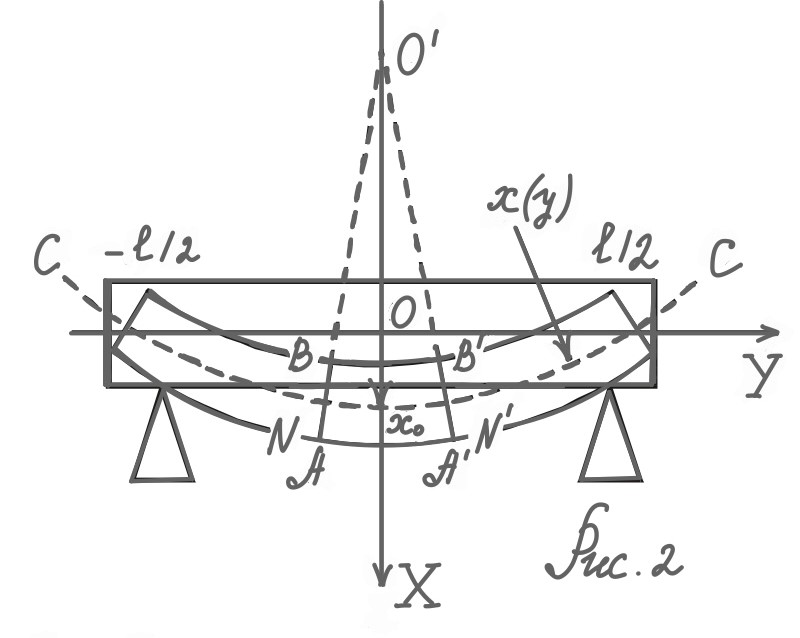
\includegraphics[width=8cm]{pictures/2.PNG}
\label{fig:image}
\end{wrapfigure}
Рассмотрим элемент $AA'B'B$. Ввиду его малости, можно считать, что кривые $AA'$, $NN'$ и $BB'$ есть дуги окружностей с центрами, лежащими на так называемой оси изгиба $O'$, перпендикулярной к плоскости рисунка. Наружная поверхность доски между точками $A$ и $A'$ при изгибе растянута, а внутренняя поверхность между точками $B$ и $B'$ - сжата. Длины кривых $AA'$ и $BB'$ в отстутствие изгиба одинаковы и равны длине $l_0$ центральной кривой $NN'$, не меняющей своей длины при изгибе доски. Пусть $R$ - радиус кривизны линии $NN'$, тогда $l_0 = R\alpha$, где $\alpha$ - центральный угол, опирающийся на дугу $NN'$. Если доска не слишком толстая, то есть $h \ll R$, длина кривой $AA'$ будет $$l_1 = \left(R + \dfrac{h}{2}\right)\alpha,$$ а ее удлинение из-за изгиба составит $$\Delta l = l_1 - l_0 = \dfrac{h\alpha}{2}.$$ Следовательно, напряжение, действующее вдоль наружной поверхности доски, согласно закону Гука, есть $$\sigma = E\dfrac{\Delta l}{l_0} = \dfrac{Eh}{2R}.$$

\section*{Приложение 2}

Найдем радиус кривизны поверхности доски в ее середине ($y = 0$) при изгибе. Заметим, что если $R$ есть радиус кривизны какой-либо кривой в данной точке, то проходящая через эту точку окружность радиусом $R$, центр которой лежит на нормали к кривой в этой точке, совпадает (по определению радиуса кривизны) с кривой в малой окрестности этой точки. Из формулы для $x(y)$ при |$\dfrac{\pi y}{l}$| $\ll$ 1 имеем $$x(y) = x_0 - \dfrac{x_0}{2}\left(\dfrac{\pi}{l}\right)^2y^2$$ (здесь использована известная приближенная формула $\cos{\gamma} = 1 - \dfrac{\gamma^2}{2!}$ для |$\gamma$| $\ll 1$). 

Искомая окружность радиусом $R$ с центром в точке $O'$(см. рис. 2), проходящая через точку с координатами $(x_0, 0)$, о которой говорилось также в Приложении 1, описывается уравнением $$y^2 + (x - x_0 + R)^2 = R^2,$$ которое легко решить относительно смещения $x(y)$: $$x(y) = x_0 - R + R\sqrt{1 - \left(\dfrac{y}{R}\right)^2}.$$ Пользуясь известной приближенной формулой $\sqrt{1 - \gamma} \approx 1 - \dfrac{\gamma}{2}$ при |$\gamma$| $\ll 1$, находим при |$\dfrac{\gamma}{R}$| $\ll 1$ $$x(y) = x_0 - \dfrac{y^2}{2R}.$$
Сравнивая два выражения для $x(y)$, получаем значения для радиуса кривизны: $$R = \left(\dfrac{l}{\pi}\right)^2 \dfrac{1}{x_0}.$$

\section*{Приложение 3}

Определим зависимость величины отклонения $x_0$ центра доски, лежащей на двух опорах, от величины приложенной к ней внешней силы $F$, распределенной вдоль центральных волокон и направленной вниз. Массой доски будем пренебрегать.

Вследствие предполагаемой симметрии, сила $F$ распределится между опорами поровну. Рассечем мысленно доску на две части, проведя нормальное сечение через центр доски (см. рис. 2), и рассмотрим условие равновесия левой половины доски. Справа на нее будет действовать внешняя сила $\dfrac{F}{2}$, сосредоточенная вблизи ее края и направленная вниз. Эта сила компенсируется силой реакции левой опоры. Сумма моментов обеих сил относительно центра доски будет, очевидно, определяться только моментом силы со стороны левой опоры: $$M = \dfrac{Fl}{4}.$$

С другой стороны, этот момент уравновешивается моментом сил растяжения и сжатия, действующих в проведенном нормальном сечении на левую часть доски со стороны правой части. Значение этого момента сил можно получить из формулы для $\sigma$, модифицировав ее для вычисления напряжения в объеме доски вдоль оси $Y$. Как следует из вывода этой формулы (см. Приложение 1), для этого достаточно вместо отклонения $\dfrac{h}{2}$ от линии $NN'$, соответствующего точке на внешней поверхности доски, ввести расстояние $\delta$ от этой линии ($-\dfrac{h}{2} < \delta < \dfrac{h}{2}$). Тогда для напряжения в объеме доски получим $$\sigma = \dfrac{E\delta}{R}.$$ Искомый момент упругих сил растяжения и сжатия относительно центра доски будет равен \[M = \int\limits_{-\dfrac{h}{2}}^{\dfrac{h}{2}}\delta \sigma d d\delta = \dfrac{E}{R}d\int\limits_{-\dfrac{h}{2}}^{\dfrac{h}{2}}\delta^2 d\delta = \dfrac{Eh^3d}{12R}\].

Подставив сюда значения радиуса кривизны $R$ и приравняв правые части двух выражений для $M$, находим связь между силой $F$ и смещением $x_0$: $$x_0 = \dfrac{3Fl^3}{\pi^2Eh^3d}.$$ Это равенство можно переписать в виде $$F = kx_0,$$ откуда следует искомое выражение для коэффициента жесткости $k$ эквивалентной пружины: $$k = \dfrac{\pi^2Eh^3d}{3l^3}.$$

\section*{Литература}
1. Научно-популярный физико-математический журнал «Квант», 1998 год, №5, А.Бирюков, "Тамэси-вари".
\begin{figure}[h]
\begin{center}
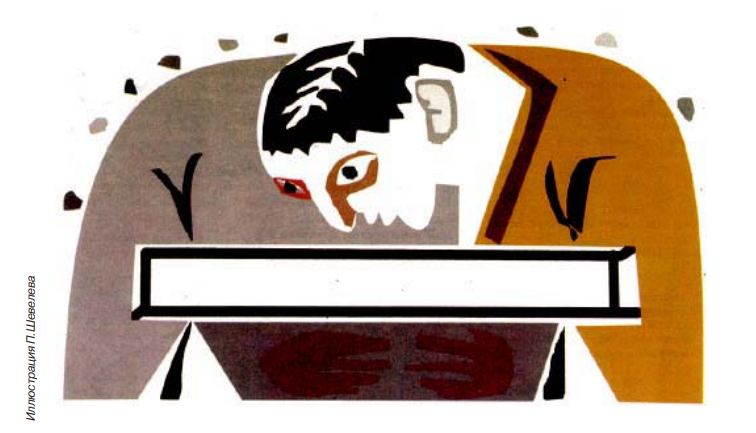
\includegraphics[width=15cm]{pictures/кек.PNG}
\label{fig:image}
\end{center}
\end{figure}
\end{document}
